% Fourier Neural Operator (FNO).  Build: latexmk -pdf fno.tex
\documentclass[border=8pt]{standalone}
\usepackage{amsmath}
% Shared TikZ palette + node styles for the ML-RT2 architecture diagrams.
% Colours match the ML-RT comparison-paper figures so the three papers look consistent:
%   pink   = data / vectors (inputs, outputs, latent representations)
%   blue   = learned networks / operators (MLPs, encoders, decoders, ...)
%   orange = special operations / physics (spectral transforms, RT residual, ...)
%   green  = loss / training terms
\usepackage{tikz}
\usetikzlibrary{arrows.meta,positioning,fit,backgrounds,calc}

\definecolor{dataFill}{HTML}{F2E6FF}\definecolor{dataDraw}{HTML}{6600CC}
\definecolor{netFill}{HTML}{B5E8E8}\definecolor{netDraw}{HTML}{086565}
\definecolor{opFill}{HTML}{FFE0C2}\definecolor{opDraw}{HTML}{AB4F03}
\definecolor{lossFill}{HTML}{C8F4C1}\definecolor{lossDraw}{HTML}{0C5600}

\tikzset{
  font=\small,
  box/.style  ={draw, rounded corners, align=center, inner sep=4pt, minimum height=9mm, line width=0.3mm},
  data/.style ={box, fill=dataFill, draw=dataDraw},
  net/.style  ={box, fill=netFill,  draw=netDraw},
  op/.style   ={box, fill=opFill,   draw=opDraw},
  loss/.style ={box, fill=lossFill, draw=lossDraw},
  sum/.style  ={draw=netDraw, circle, inner sep=1.3pt, fill=white, line width=0.3mm},
  arr/.style  ={-{Stealth[length=2.4mm]}, thick},
  darr/.style ={-{Stealth[length=2.4mm]}, thick, dashed},
  note/.style ={align=center, font=\scriptsize, text=black!65},
}

\begin{document}
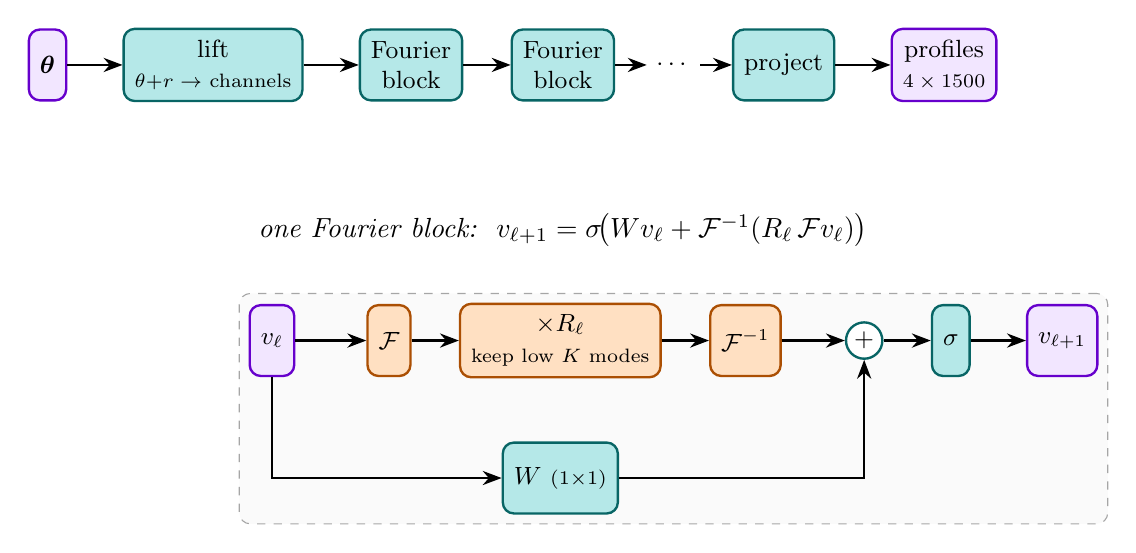
\begin{tikzpicture}[node distance=7mm]
  % top-level flow
  \node[data]                (in)   {$\boldsymbol{\theta}$};
  \node[net,  right=of in]   (lift) {lift\\{\scriptsize $\theta{+}r\to$ channels}};
  \node[net,  right=of lift] (f1)   {Fourier\\block};
  \node[net,  right=6mm of f1] (f2)  {Fourier\\block};
  \node[right=4mm of f2]     (dots) {$\cdots$};
  \node[net,  right=4mm of dots] (proj) {project};
  \node[data, right=of proj] (out)  {profiles\\{\scriptsize $4\times1500$}};
  \foreach \a/\b in {in/lift, lift/f1, f1/f2, f2/dots, dots/proj, proj/out}
      \draw[arr] (\a) -- (\b);

  % expanded Fourier block
  \node[below=13mm of f2, font=\itshape]
        (cap) {one Fourier block:\ \ $v_{\ell+1}=\sigma\!\big(W v_\ell + \mathcal{F}^{-1}(R_\ell\,\mathcal{F} v_\ell)\big)$};
  \node[data, below=6mm of cap.south west, anchor=north west] (v) {$v_\ell$};
  \node[op,   right=9mm of v]    (fft)  {$\mathcal{F}$};
  \node[op,   right=6mm of fft]  (R)    {$\times R_\ell$\\{\scriptsize keep low $K$ modes}};
  \node[op,   right=6mm of R]    (ifft) {$\mathcal{F}^{-1}$};
  \node[net,  below=8mm of R]    (W)    {$W$\ {\scriptsize (1$\times$1)}};
  \node[sum,  right=8mm of ifft] (plus) {$+$};
  \node[net,  right=6mm of plus] (act)  {$\sigma$};
  \node[data, right=7mm of act]  (vo)   {$v_{\ell+1}$};
  \draw[arr] (v) -- (fft);   \draw[arr] (fft) -- (R);   \draw[arr] (R) -- (ifft);
  \draw[arr] (ifft) -- (plus);
  \draw[arr] (v.south) |- (W);  \draw[arr] (W) -| (plus);
  \draw[arr] (plus) -- (act);  \draw[arr] (act) -- (vo);
  \begin{scope}[on background layer]
    \node[draw=black!35, dashed, rounded corners, fill=black!2,
          fit=(v)(fft)(R)(ifft)(W)(plus)(act)(vo)] {};
  \end{scope}
\end{tikzpicture}
\end{document}
